\documentclass{article}
\usepackage{graphicx} % Required for inserting images
\usepackage{amsmath}
\usepackage{amssymb}
\usepackage{indentfirst}
\usepackage{float}
\usepackage{caption}
\usepackage{enumitem}
\usepackage[a4paper, total={6in, 10in}]{geometry}
\setlength{\arraycolsep}{0.1cm}
\title{Mathcamp 2026 Qualifying Quiz Problem 5 Solution}
\author{Applicant ID: 25107}
\date{}

\begin{document}
	
	\maketitle
	
	\section*{Part a)}
    First, note that updating a digit $m$ times increases it by $1$ modulo $k$. Assume the starting digit is $d$. If $d < k - 1$, then $d + 1 \equiv d \pmod k$, and if $d = k - 1,$ then $0 \equiv k\pmod k$. So, starting from $d$ simply makes the digit $d + m$ modulo $k$. 
    
    To reach $k^n$ different strings, we must perform $k^n - 1$ moves. If a digit is increased $m$ times, then the final digit $d$ satisfies $m\equiv d\pmod k$. The final digit sum is $n(k - 1)$, therefore, we must have
    $$k^n - 1\equiv n(k - 1) \pmod k$$
    $$-1\equiv -n \pmod k \implies n\equiv 1\pmod k.$$
    We claim that this condition is sufficient. \\
    
    \textbf{Lemma 1:} Let $a = a_1a_2a_3\cdots a_m$ be a string of $m$ digits modulo $k$. For every $m$, there is a sequence of $k^m - 1$ moves that reaches each $m$-digit string exactly once, starting at $a$ and ending at $(a_1 - 1)a_2a_3\cdots a_m$.
    
    \textit{Proof:} We proceed by induction on $m$. For the base case $m = 1$, incrementing the single digit $k - 1$ times reaches all $k$ digits, ending at $a_1 + k - 1 \equiv a_1 - 1\pmod k$.

    For the inductive step, assume Lemma 1 holds for some integer $m$, and consider an $(m + 1)$-digit string $a_1a_2\cdots a_{m + 1}$. This means there exists a sequence of moves $F_m$ of length $k^m - 1$ on the positions $1, 2, \dots, m$, which will reach every $m$-digit string on those positions, ending at $(a_1 - 1)a_2\cdots a_m$. Let $F'_m$ denote the same sequence of moves applied to positions $2, 3, \dots, m + 1$. Now consider the sequence
    $$F_{m + 1} = (F_m', 1, F_m', 1, F_m', \dots, 1, F_m'),$$
    where $F_m'$ is applied a total of $k$ times and between each such sequence we increment the first digit. Initially the first digit is $a_1$. After $a$ repetitions of $F_m'$ and first-digit increments, the first digit is equal to $a_1 + a \equiv A\pmod k$. By the inductive hypothesis, each time we apply $F_m'$, we cycle through all the length-$m$ suffixes (with first digit fixed) exactly once, so all the strings we reach with the above sequence are distinct. 
    The final string has first digit $a_1 + (k - 1)\equiv a_1 - 1\pmod k$ and the other digits are $$(a_2 - 1 - 1 - \cdots - 1)a_3a_4\cdots a_{m + 1} = (a_2 - k)a_3a_4\cdots a_{m + 1} = a_2a_3a_4\cdots a_{m + 1}$$
    modulo $k$, as required. This completes the induction. $\square$\\

    Now, let $S^n$ be the concatenation of $n$ copies of $S$, e.g. $(10)^3 = 101010$, and let $K = k^k$.
    
    \textbf{Lemma 2:} For all $m\geq 1$, there is a sequence of $K^m - 1$ moves that reaches each $mk$-digit string exactly once, starting from $0^{km}$ and ending at $((k - 1)\cdot 0^{k - 1})^m$.

    \textit{Proof:} We proceed by induction on $m$. The base case $m = 1$ is clear from Lemma 1, which allows us to transform from $0^k$ to $(k - 1)\cdot 0^{k - 1}$ using a sequence of moves $B = (b_1, b_2, \dots, b_{K - 1})$.

    For the inductive step, assume Lemma 2 holds for some integer $m$ with some sequence of moves $G_m$, and consider the case of a length-$(m + 1)k$ string. View the string as $m + 1$ blocks of $k$ digits. Let $G'_m$ be the same sequence as $G_m$, but applied to blocks $2, 3, \dots, m + 1$. Now, consider the sequence $$G_{m + 1} = (G_m', b_1, G_m', b_2, G_m', \dots, b_{K - 1}, G'_m),$$
    so that $G'_m$ is applied $K$ times. Since $G_m'$ only affects blocks $2$ to $m + 1$, each application of $G_m'$ reaches all possible suffixes for the current string in the first block. Therefore, going through the sequence, we will reach all combinations suffixes with block 1 prefixes, so we will reach all length-$(m + 1)k$ strings exactly once. The ending string will be $$((k - 1)\cdot 0^{k - 1})\cdot ((k - 1)\cdot 0^{k - 1})^m = ((k - 1)\cdot 0^{k - 1})^m,$$
    as desired, completing the induction. $\square$\\

    Finally, we construct the sequence of moves for $n\equiv 1 \pmod k$. Let $n = mk + 1$ for some integer $m$. Consider the sequence of moves $G_m$ described in Lemma 2. Notice that by permuting the digit labels by increasing each label by $a$ modulo $k$, we can display all $K^m$ strings exactly once, but ending at $(0^{a}(k - 1)0^{k - a - 1})^m$. Let this family of sequences be $H_{m, a}$. Consider the following sequence of moves:
    $$H_{m, 1}, n, H_{m, 2}, n,H_{m, 3}, \dots, n, H_{m, k}$$
    We can see that $H_{m, 1}$ lists all $K^m$ strings ending with $0$, then incrementing the last digit and applying $H_{m, 2}$ lists all $K^m$ strings ending with $1$, etc. At the end, the last digit has been incremented $k - 1$ times, while the $H_{m, a}$ operations make all digits in the $k$-blocks equal to $(k - 1)$. Therefore, the final string is $(k - 1)^n$, as desired.

    \section*{Part b)}

    The problem can be rephrased as follows:

    There is a directed graph of $k^2$ vertices, where each vertex has coordinates $(x, y)$ with $0\leq x, y < k$. Each vertex $(x, y)$ has a directed edge to $(x + 1, y)$ and $(x, y + 1)$, where coordinates are taken modulo $k$. Call these edges the vertex's $x$-edge and $y$-edge respectively. Starting at $(0, 0)$, we wish to find all possible endings of a Hamiltonian path on this graph.

    First, notice that each move increases $x + y$ by one modulo $k$. Since we perform $k^2 - 1$ moves, we see that the ending vertex must satisfy $x + y\equiv k^2 - 1 \equiv k - 1\pmod k$, which are the vertices on the main diagonal opposite $(0, 0)$.

    Consider a valid Hamiltonian path on this graph, ending at $v_d = (d, k - 1 - d).$ Each vertex except for $v_d$ has outwards degree 1, and each vertex except for $(0, 0)$ has inwards degree $1$. Let the diagonals be defined as $$D_t = \{(x, y)\ |\ x + y\equiv t\pmod k\},\ 0\leq t < k.$$

    Notice that $v_d$ lies on diagonal $D_{k - 1}$. First, assume $d > 0$, so $v_d\neq v_0$, and consider the outgoing edge from $v_0 = (0, k - 1)$. Since $(0, 0)$ has in-degree $0$, $v_0$ must use the $x$-edge, so $(1, k - 1)$ has in-degree $1$. Since the Hamiltonian path cannot enter $(1, k - 1)$ again, this forces $v_1$ to use the $x$-edge also. We can continue this argument to see that for $0\leq t < d$, $v_t$ uses the $x$-edge. Similarly, for $d < t < k$, $v_t$ uses the $y$-edge.

    Also, by the same vertex degree argument, we can see that the vertices in each diagonal either all use the $x$-edge or all use the $y$-edge: the edges from $D_i$ to $D_{i + 1}$ (where $i < k - 1)$ must form a bijection between the vertices in the two diagonals. 
\begin{figure}[h]
    \centering
    \vspace{-0.3cm}
    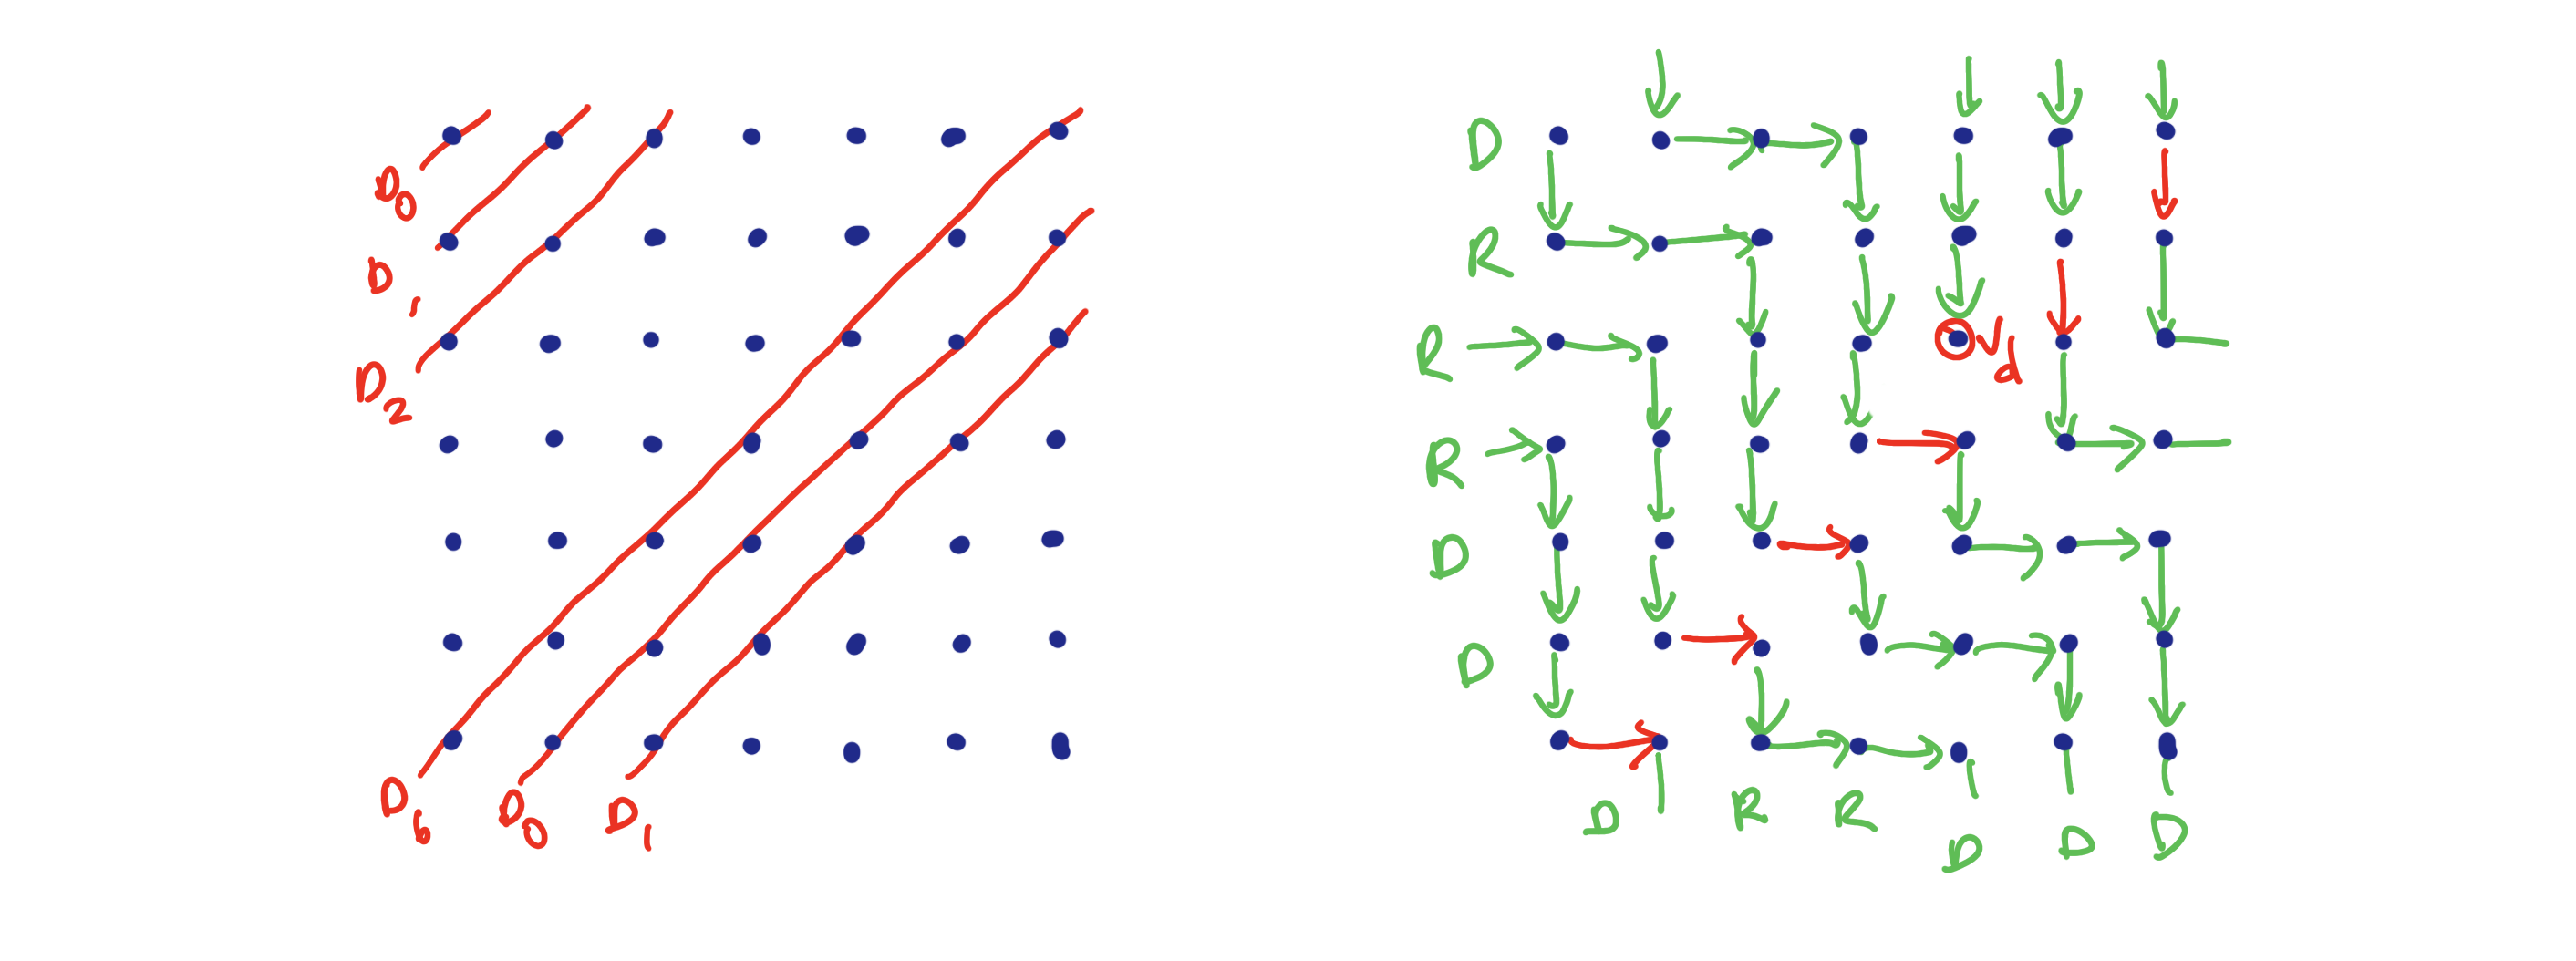
\includegraphics[width=15cm, trim = 2 0.5cm 2 0.5cm, clip]{diagonal.png}
    \vspace{-0.3cm}
\end{figure}
    
    Let $X$ be the number of diagonals from $D_0, D_1, \dots, D_{k - 2}$ that use $x$-edges, and let $d$ be defined identically as before (determining the ending vertex). When traversing $D_0, D_1, \dots, D_{k - 2}$, we always increase our $x$-coordinate by $X$, so we can construct the following sequence $x_i$, where $x_i$ tracks our $x$-coordinate the $i$-th time we reach a vertex in $D_{k - 1}$:
    \begin{enumerate}[itemsep=0mm]
    \item $x_1 = X$, and $0\leq x_i< k$ for all $i$.
    \item For $i \geq 1$:
    \subitem if $x_i < d$, then $x_{i + 1} \equiv x_i + 1 + X\pmod k$. 
    \subitem if $x_i > d,$ then $x_{i + 1} \equiv x_i + X\pmod k$. 
    \subitem if $x_i = d$, the sequence ends as we have reached the target (so $x_{i + 1}$ is not defined).
    \end{enumerate}    
    
    To verify whether $v_d$ is a possible ending vertex for a Hamiltonian path, we wish to determine whether there exists $X$ such that the sequence ends at $x_k$ (thus reaching all vertices). Since all vertices in $D_{k - 1}$ have distinct $x$-coordinates, we see that $x_1, x_2, \dots, x_k$ must be a cyclic permutation of $\{0, 1, 2,\dots, k - 1\}$. Specifically, we can write it as a composition of two permutations: first, to add one to all elements less than $d$ (and send $d$ to $0$ to satisfy being a permutation), and second, one that represents addition of $X$ modulo $k$. We can use Cauchy's two-line notation to write our permutations, where the initial elements are listed in the top row and their respective images are listed in the bottom row (modulo $k$):
    $$\begin{pmatrix} 
    x_1 & x_2 & \cdots & x_k \\
    x_2 & x_3 & \cdots & x_1 \end{pmatrix} = 
    \begin{pmatrix} 
    0 & 1 & \cdots & d - 1 & d & d + 1 & \cdots & k - 1 \\
    1 & 2 & \cdots & d & 0 & d + 1 & \cdots & k - 1 \end{pmatrix} 
    \begin{pmatrix} 
    0 & 1 & \cdots & k - 1 \\
    X & X + 1 & \cdots & X + k - 1\end{pmatrix}$$
    
    Observe the signs of the permutations. Since the left-hand side is a cycle of length $k$, it has sign $(-1)^{k - 1}$. The left permutation on the right-hand side contains a cycle of length $d + 1$, so it has sign $(-1)^d$. Finally, the rightmost permutation will form $\gcd(k, X)$ disjoint cycles, each of length $\frac{k}{\gcd(k, X)}.$ Therefore, its sign will be $$\left((-1)^{\frac{k}{\gcd(k, X)} - 1}\right)^{\gcd(k, X)} = (-1)^{k - \gcd(k, X)}.$$
    Since the sign of a permutation is multiplicative, we have $(-1)^{k - 1} = (-1)^{d + k - \gcd(k, X)}$, which gives
    $$d - \gcd(k, X)\equiv 1 \pmod{2}.$$
    If $k$ is even, then $\gcd(k, X)$ can be either parity, so $d$ can have either parity. When $k$ is odd, $\gcd(k, X)$ is always odd, so $d$ must be even. \\

    We now construct a valid Hamiltonian path that ends at all possible shown $v_d$ by selecting suitable $X$.

    \textbf{Case 1:} $k$ is odd.

    As found above, we can only reach $v_d$ when $d$ is even. Consider $X = 1$. Following the definition of $x_i$, the sequence $x_1, x_2, \dots$ will increase by $2$ whenever $x_i < d$, and increase by $1$ (modulo $k$) whenever $x_i > d$, yielding:
    $$1, 3, 5, \dots, d - 1, d + 1, d + 2, d + 3, \dots, k - 1, 0, 2, 4, \dots, d.$$
    The sequence forms a permutation of $0, 1, \dots, k - 1$, so setting $X = 1$ produces valid Hamiltonian paths to each ending vertex $v_d$ for even $d$.

    \textbf{Case 2:} $k$ is even.
    
    \textbf{Subcase 2.1:} $d$ is even.
    
    Once again, consider $X = 1$, and follow the steps to produce the sequence $x_i$:
    $$1, 3, 5, \dots, d - 1, d + 1, d + 2, d + 3, \dots, k - 1, 0, 2, 4, \dots, d.$$
    The sequence forms a permutation of $0, 1, \dots, k - 1$, so setting $X = 1$ produces valid Hamiltonian paths to each ending vertex $v_d$ for even d.

    \textbf{Subcase 2.2:} $d$ is odd.

    Consider $X = k - 2$. Following the definition of $x_i$, the sequence $x_1, x_2, \dots$ will decrease by $2$ (increase by $k - 2\pmod k$) whenever $x_i > d$, and decrease by $1$ modulo $k$ (increase by $k - 2 + 1\pmod k$) whenever $x_i < d$, yielding: 
    $$k - 2, k - 4, k - 6, \dots, d + 1, d - 1, d - 2, d - 3, \dots, 1, 0, k - 1, k - 3, k - 5, \dots, d.$$
    The sequence forms a permutation of $0, 1, \dots, k - 1$, so setting $X = k - 2$ produces valid Hamiltonian paths to each ending vertex $v_d$ for odd d.

    This finishes the construction. To conclude, the possible ending digits are all pairs of the form $(d, k - 1 - d)$ for $0\leq d < k$, where $d$ additionally must be even if $k$ is odd.

    Some example paths are shown below, using the values of $X$ given above:

    \begin{figure}[H]
    \centering
    \vspace{-0.3cm}
    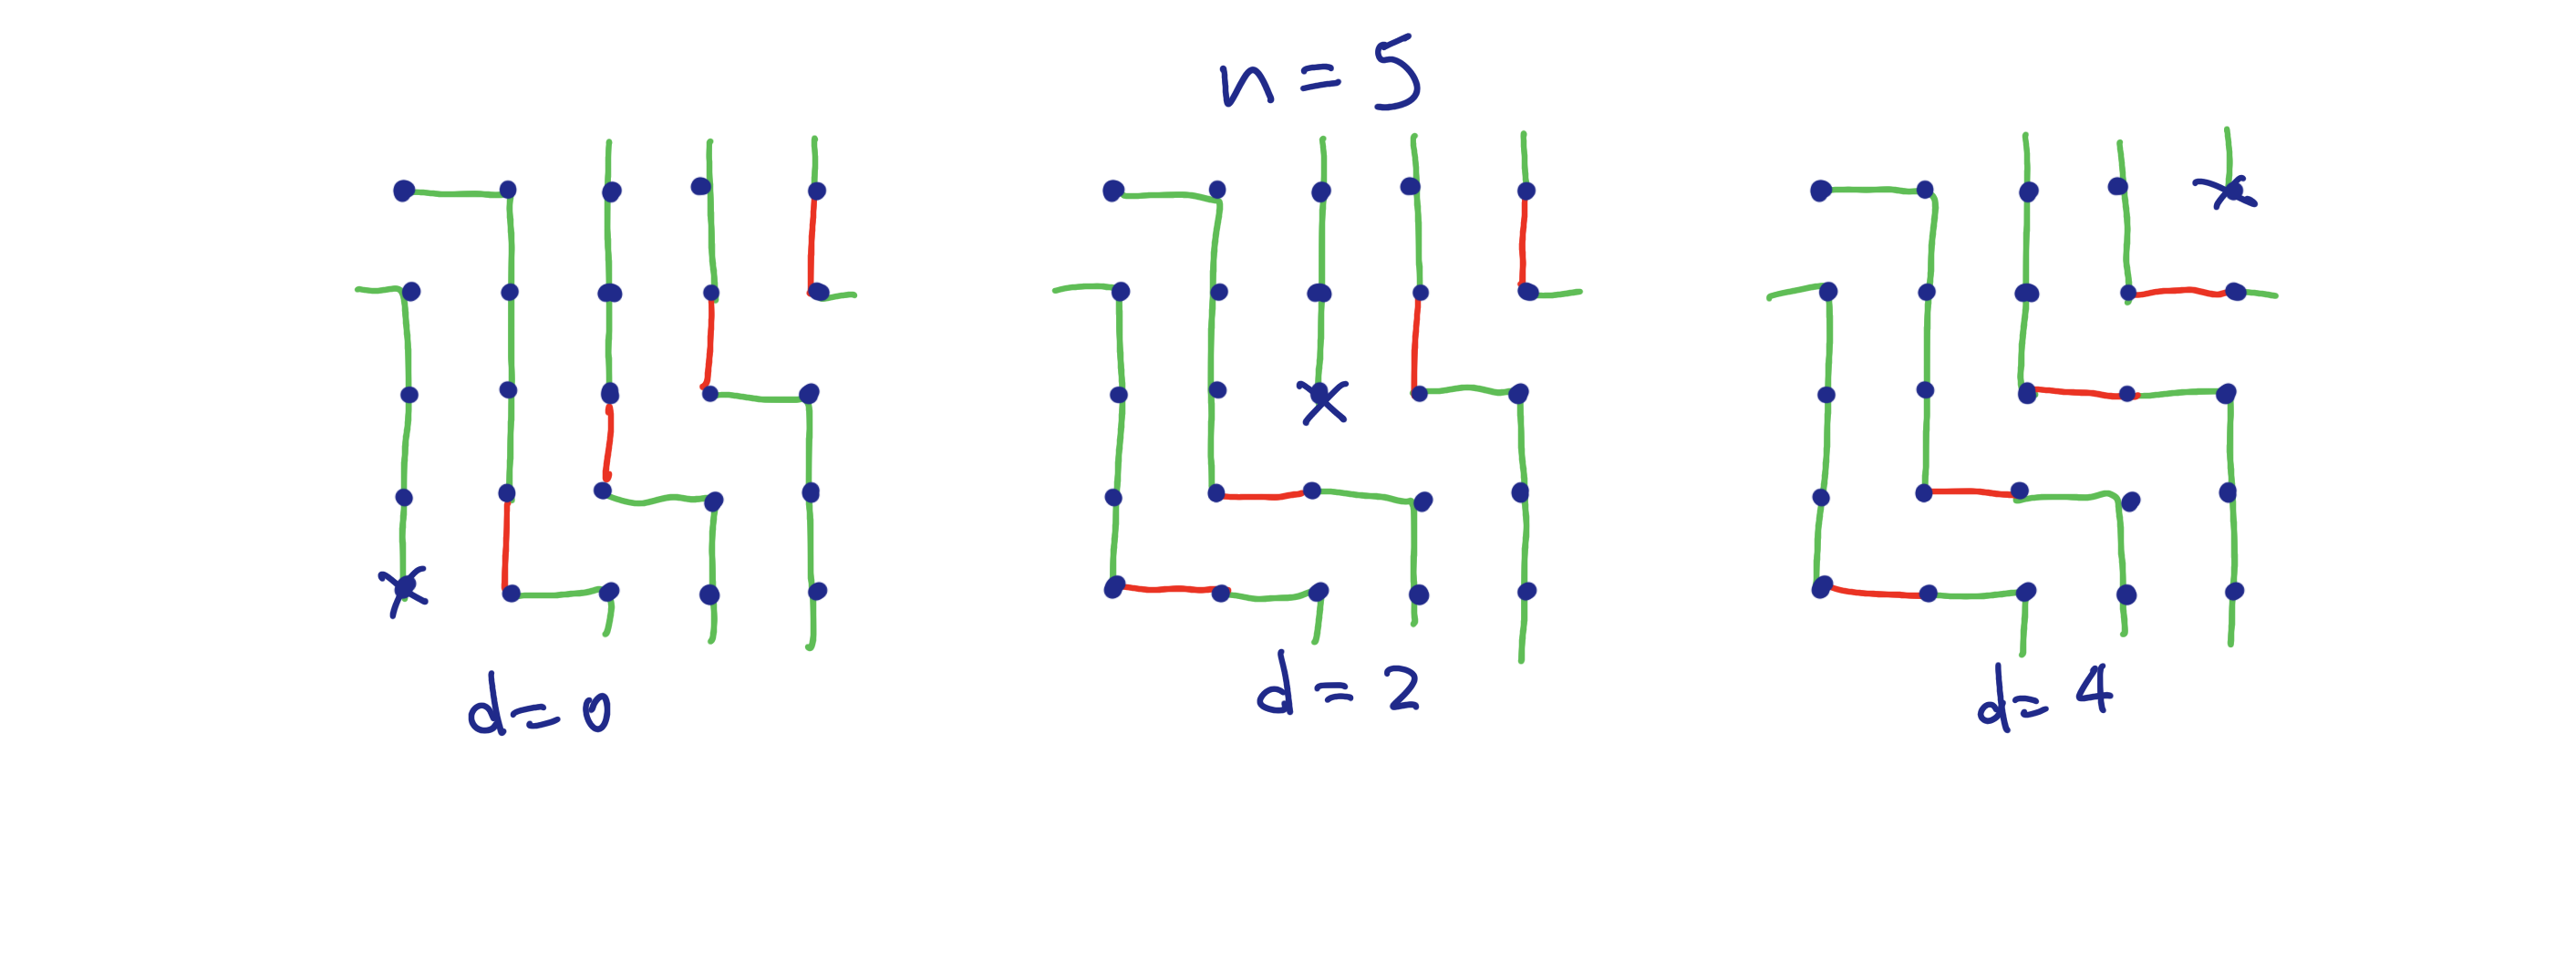
\includegraphics[width=15cm, trim = 3cm 2cm 3cm 0cm, clip]{example1.png}
    \vspace{-0.3cm}
    \end{figure}
    
    \begin{figure}[H]
    \centering
    \vspace{-0.3cm}
    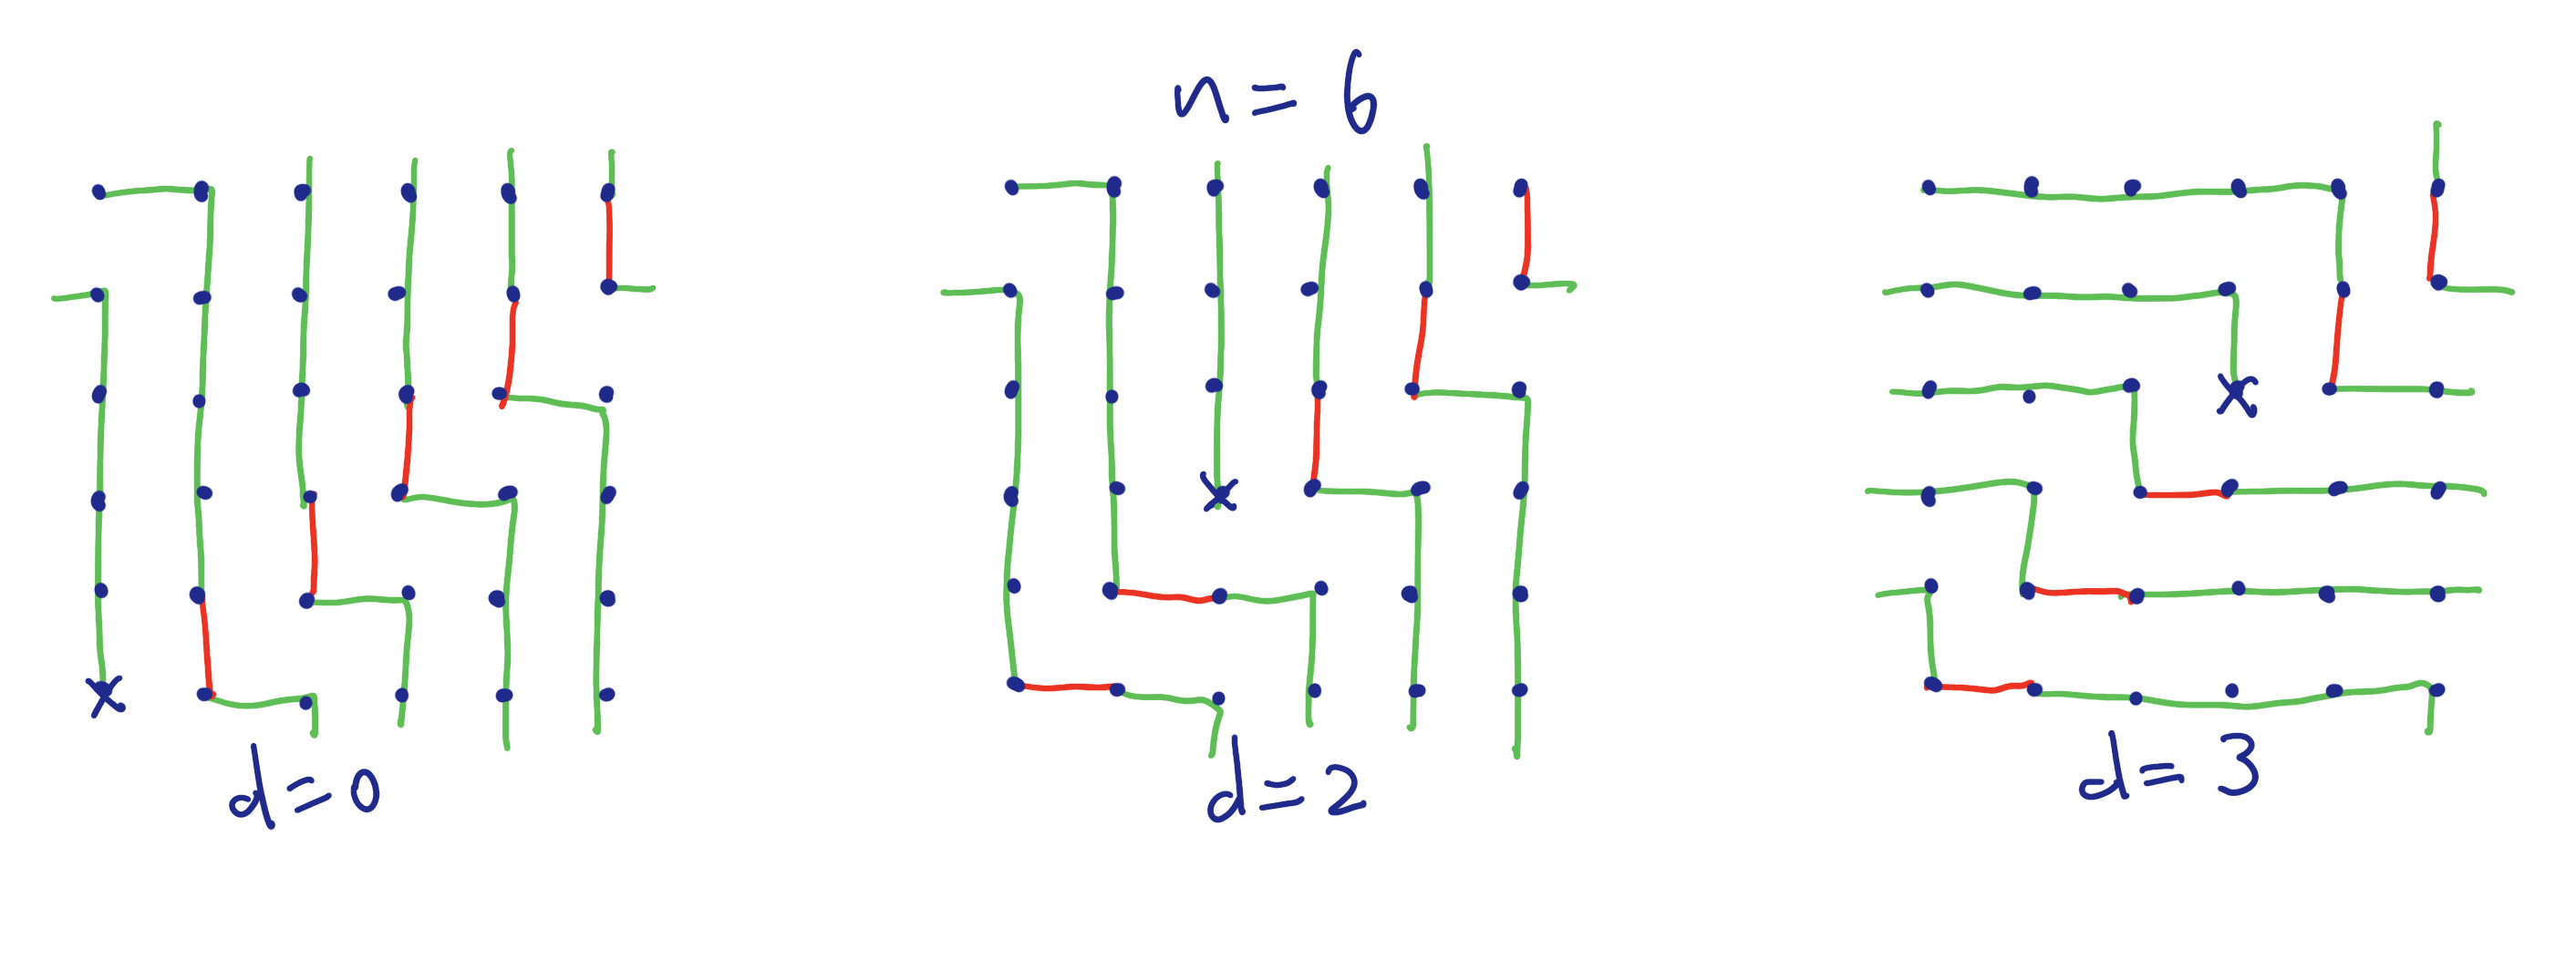
\includegraphics[width=15cm, trim = 0 0cm 0 0.5cm, clip]{example2.png}
    \vspace{-0.3cm}
\end{figure}
\end{document}